%%*****************************************************************************
%% $Id: started.tex,v 0.00 2008/05/01 17:52:50 gene Exp $
%%*****************************************************************************
%% Author: Gerd Neugebauer
%%-----------------------------------------------------------------------------

\chapter{Getting Started}
%@author Gerd Neugebauer

In this chapter we describe the steps you can take to get \ExBib\ up
and running. We try to use as few as possible premises. Thus it should
be not too hard to get started.

\section{Prerequisites}
%@author Gerd Neugebauer

\subsection{Java}%
\index{Java|(}
%@author Gerd Neugebauer

You need to have Java 5\index{Java} or later installed on your
system. You can get Java for a several systems directly from
\url{java.sun.com}. Download and install it according to the
installation instructions for your environment.

To check that you have an appropriate Java on your path you can use
the command \texttt{java} with the argument \texttt{-version}. This
can be seen in the following example:

\lstset{morecomment=[l]{\#}}%
\begin{lstlisting}{morecomment=[l][keywordstyle]{>}}
# java -version
java version "1.5.0_04"
Java(TM) 2 Runtime Environment, Standard Edition (build 1.5.0_04-b05)
Java HotSpot(TM) Client VM (build 1.5.0_04-b05, mixed mode)
#
\end{lstlisting}
\index{Java|)}


\subsection{TEXMF}%
%@author Gerd Neugebauer
\index{TEXMF|(}

If you want to use more than the pure \ExBib\ engine, styles can be
inherited from a texmf tree\index{texmf}. \ExBib\ itself does not
contain a full texmf tree. It comes just with some rudimentary files
necessary for testing and getting started. Thus you should have
installed a texmf tree, e.g. from a \TeX Live\index{TeXlive@\TeX Live}
installation. This can be found on the
\href{http://www.ctan.org}{Comprehensive \TeX\ Archive Network
  (CTAN)}\index{CTAN}.

There is no need to install the texmf tree in a special place. You
have to tell \ExBib\ anyhow where it can be found. It is even possible
to work with several texmf trees.

One requirement for the texmf trees is that they have a file database
(\File{ls-R}). \ExBib\ can be configured to work without it, but then
\ExBib\ is deadly slow. Thus you do not really want to try this
alternative.
\index{TEXMF|)}

\section{Getting \ExBib}
%@author Gerd Neugebauer

\subsection{Getting the Installer}
%@author Gerd Neugebauer

The simplest way to get \ExBib\ up and running is to use the \ExBib\ 
installer. This installer\index{installer} is distributed as one file
\File{ExBib-setup.jar}. You can download it from

\begin{quotation}
  \url{http://www.extex.org/download/}
\end{quotation}

If you have got the installer there is no need for you to get the
sources as well. Nevertheless the soruces can be retrieved via
Subversion from
\begin{quotation}
  \url{https://svn.berlios.de/svnroot/repos/extex/trunk/ExBib}
\end{quotation}


\section{Installing \ExBib}\label{sec:install}
%@author Gerd Neugebauer

The installation of \ExBib\ works with the \ExBib\ installer. This
installer is named \File{ExBib-setup.jar}. You can start the installer
with the following command line:\index{installer}

\begin{lstlisting}{}
# java -jar ExBib-setup.jar
\end{lstlisting}

On Windows\index{Windows} with a properly installed Java\index{Java}
you can also start the installer by double-clicking
\File{ExBib-setup.jar} in the Explorer\index{Explorer}. This might
work on other windowing systems as well.

\begin{figure}[!ht]
  \centering
  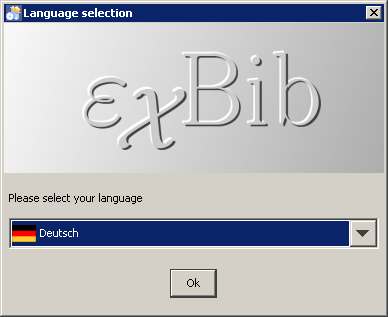
\includegraphics[width=.45\textwidth]{img/inst1}\hfill
  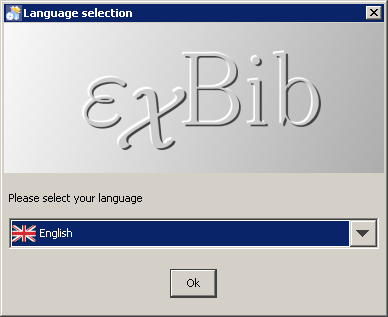
\includegraphics[width=.45\textwidth]{img/inst2}
  \caption{The Language Selection in the Installer}
  \label{fig:inst1}
\end{figure}
The installer provides a graphical user interface with a wizard
guiding you through the installation process. The first dialog is
shown in figure~\ref{fig:inst1}. As you can see you can select one of
several languages for the installation process. This selection just
effects the language used to communicate during the instanllation
process.  Currently the languages English and German are supported.
There might be some more at the time you are performing the
installation.\index{installer!language}\index{language!installer}

Note that the language selection covers the installer only. \ExBib\ 
can be run under different language environments as well. This is
controlled by a setting at run-time. Currently only an English and
a German language binding for \ExBib\ are provided.\index{language}

\begin{figure}[!ht]
  \centering
  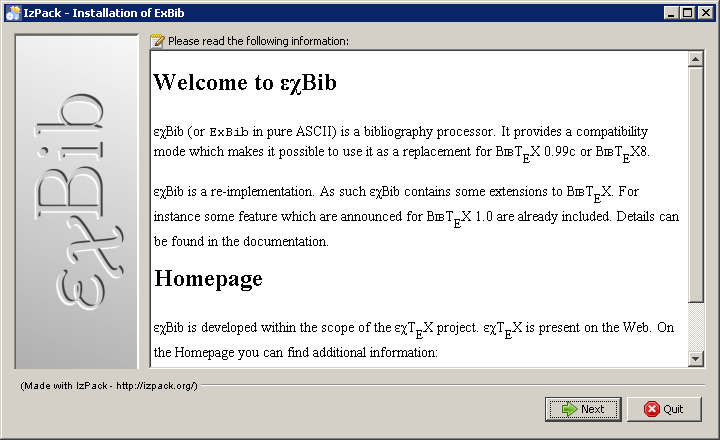
\includegraphics[width=.45\textwidth]{img/inst3}
  \caption{Welcome to \ExBib}
  \label{fig:inst2}
\end{figure}

The next panel shows a welcome message showing what this installer is
about (see figure~\ref{fig:inst2}). Since you are reading this
document there is nothing new for you.

\begin{figure}[!ht]
  \centering
  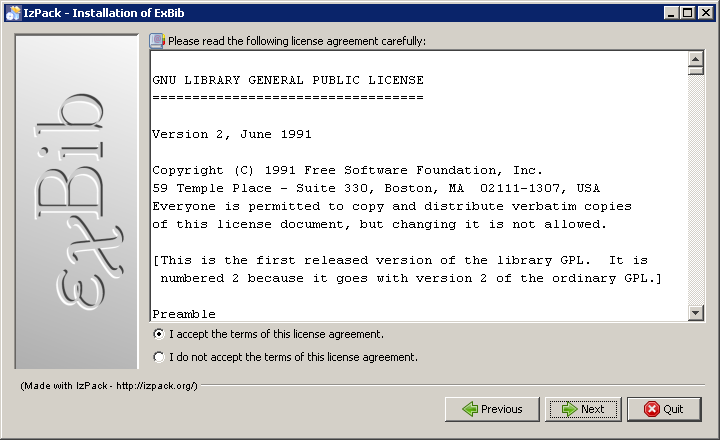
\includegraphics[width=.45\textwidth]{img/inst4}
  \caption{Accepting the Licence}
  \label{fig:inst3}
\end{figure}

Now the license\index{license} of \ExBib\ is presented (see
figure~\ref{fig:inst3}). It is there to remind you that there is
something like a license. You can not do everything with the software.
But the limitations are very minimalistic. Usually it should not
really affect you -- especially when you are migrating from \BibTeX.

Note that the license is the LGPL\index{LGPL}\index{license!LGPL}. In
contrast to the GPL\index{GPL}\index{license!GPL} it does not infect
other software build from \ExBib\ or containing it.

\begin{figure}[!ht]
  \centering
  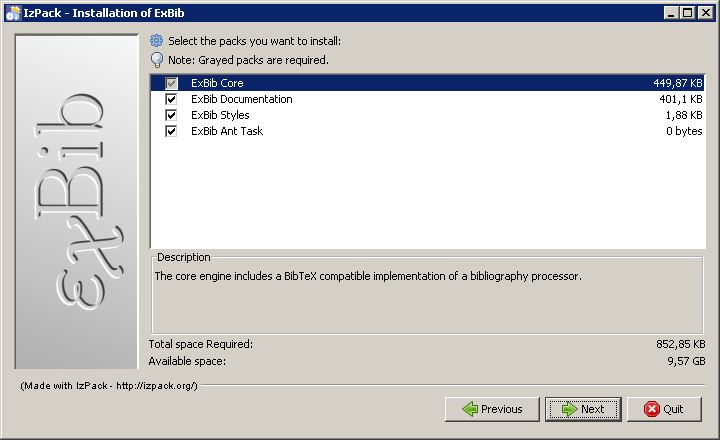
\includegraphics[width=.45\textwidth]{img/inst5}
  \caption{Selecting the Packages}
  \label{fig:inst4}
\end{figure}

Next the packages to be installed can be selected (see
figure~\ref{fig:inst4}). The core packages is needed in any case. Thus
it can not be deselected. The other packages can be freely choosen
from.

Whenever you select a package in the list a short discription of the
package is displayed.

\begin{figure}[!ht]
  \centering
  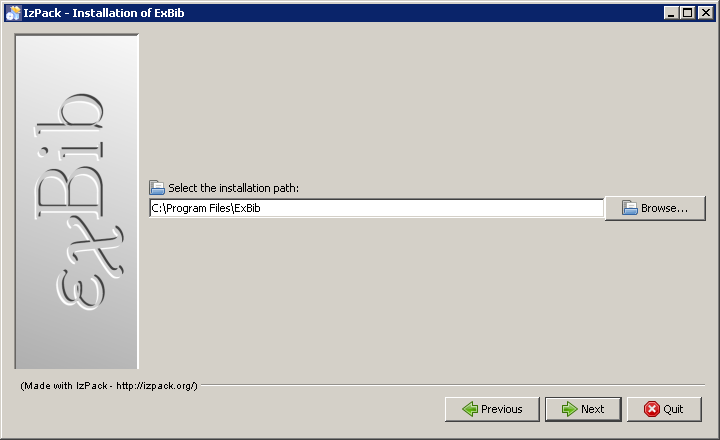
\includegraphics[width=.45\textwidth]{img/inst6}
  \caption{Selecting the Installation Directory}
  \label{fig:inst5}
\end{figure}

Finally the installation directory\index{installation
  directory}\index{directory installation} has to be selected (see
figure~\ref{fig:inst5}). The installation directory (see also
section~\ref{sec:inst.dir}) is the only directory the \ExBib\ 
installer creates files in. Usually is should be separate from other
directories. For instance the value \verb|C:\Program Files\ExBib| on
Windows\index{Windows} or \verb|/opt/ExBib| on Unix\index{Unix} are
sensible values. Nevertheless the installation can also be performed
in your home directory if you do not have writing permissions in the
global directories.

This is the last decision you have to make.

\begin{figure}[!ht]
  \centering
  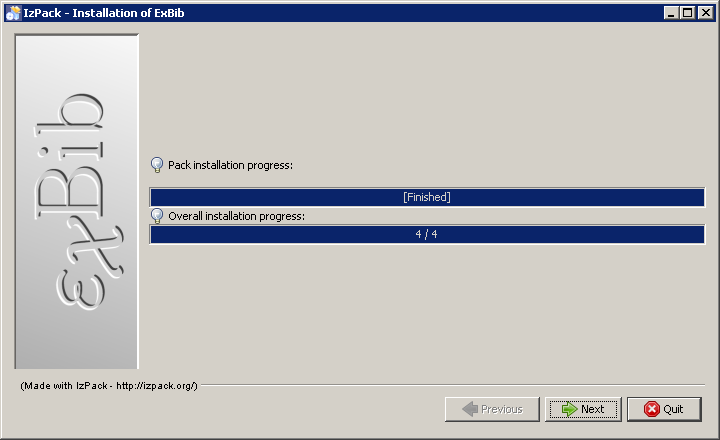
\includegraphics[width=.45\textwidth]{img/inst7}
  \caption{Progress of the Installation}
  \label{fig:inst6}
\end{figure}

Now the installation is performed. A progress panel is shown during
the installation (see figure~\ref{fig:inst6}). As a result the
installation directory is created and filled (see also
section~\ref{sec:inst.dir})

\begin{figure}[!ht]
  \centering
  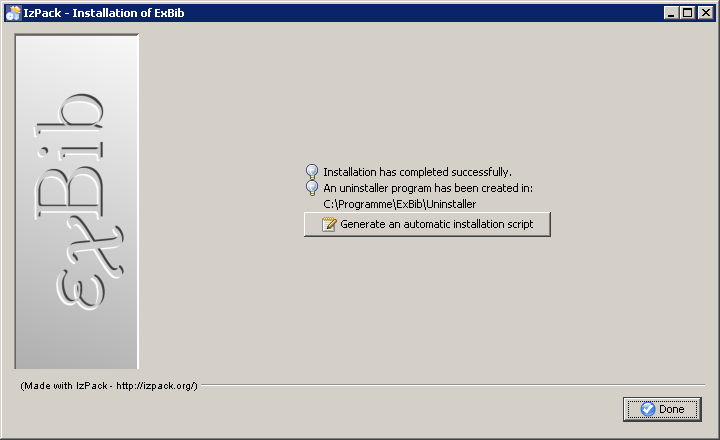
\includegraphics[width=.45\textwidth]{img/inst8}
  \caption{Saving the Installation Settings}
  \label{fig:inst7}
\end{figure}

When the installation is completed you get the chance to save the
settings for unattended replay (see figure~\ref{fig:inst7}). See
section~\ref{sec:replay} for details.


Finally you have to make sure that the executables \Prog{exbib} or
\Prog{exbib.bat} are on your path for executables.\index{path} This
can be achieved by modifying the environment variable \verb|PATH| in a
Unix environment or setting \verb|path| in the system settings on
Windows.


\subsection{The Installation Directory}\label{sec:inst.dir}
%@author Gerd Neugebauer
\index{installation directory|(}\index{directory installation|(}

During the installation you choose a directory where \ExBib\ lives.
This is called the installation directory. An example of the contents of the
installation directory can be seen in figure~\ref{fig:inst.dir}.

\begin{figure}[!ht]
  \centering
\begin{DirList}{200pt}{250pt}
  \TOPDIR(0,30){ExBib}
  \DIR(3,28)2{Uninstaller}
  \FILE(6,26)2{uninstaller.jar}
  \DIR(3,24){4.75}{bin}
  \FILE(6,22)2{exbib}
  \FILE(6,20){2.5}{exbib.bat}
  \FILE(6,18){2.5}{exbibutil}
  \FILE(6,16){2.5}{exbibutil.bat}
  \DIR(3,14){10.75}{doc}
  \FILE(6,12)2{exbib-manual.pdf}
  \DIR(3,10){4.75}{lib}
  \FILE(6,8){2}{ExBib-core.jar}
  \FILE(6,6){2.5}{ExBib-Main.jar}
  \FILE(6,4){2.5}{ExBib-styles.jar}
  \FILE(6,2){2.5}{ExTeX-resource.jar}
  \FILE(3,0){10.75}{LICENSE.txt}
\end{DirList}
  \caption{The Installation Directory}

  \label{fig:inst.dir}
\end{figure}

The directory \File{Uninstaller} contains the uninstaller. It can be
used to get rid of \ExBib\ -- even when I don't know why you should
want to. For details see section~\ref{sec:uninst}

The directory \File{bin} contains the binaries. This directory should
be put onto the path for executables. Note that currently all
executables are installed on any platform. On Windows the programs
without extension can be useful within the cygwin world. On Unix the
files with the extension \verb|.bat| can be simply ignored.

The directory \File{doc} contains documentation if the documentation
package has been selected during the installation.

The directory \File{lib} contains the libraries used by \ExBib.

\index{installation directory|)}\index{directory installation|)}

\subsection{Replaying an Installation}\label{sec:replay}
%@author Gerd Neugebauer

Sometimes it is desirable to perform an installation on several
similar machines. This means that the answers to the questions in the
installer are the same. This process can be automated.

In figure~\ref{fig:inst7} you can see the last screen of the
installer. Here you have the possibility to select the button
``Generate an automatic installation script''. This produces an XML
file which can be passed to the installer to avoid the
dialogs.\index{installer}\index{installation script}

Suppose you have named the file \texttt{replay.xml} in the file
selector which pops up when the button has been pressed. Then you can
replay the installation with the following command invocation:

\begin{lstlisting}{}
# java -jar ExBib-setup.jar replay.xml
\end{lstlisting}

This supposes that the two files \File{ExBib-setup.jar} and
\texttt{replay.xml} are in the current directory.

\subsection{Uninstalling \ExBib}\label{sec:uninst}
%@author Gerd Neugebauer

The files installed by the installer (see section~\ref{sec:install})
can be removed from the system. For this purpose an uninstaller is
provided in the subdirectory \File{Uninstaller} of the \ExBib\
installation directory. It is named \File{uninstaller.jar}. It can be
invoked by double clicking or invoking it on the command line as follows:

\begin{lstlisting}{}
# java -jar uninstaller.jar
\end{lstlisting}

\begin{figure}[!ht]
  \centering
  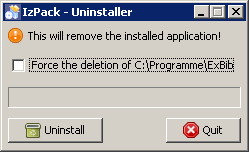
\includegraphics[width=.45\textwidth]{img/uninst1}
  \caption{Confirming the Uninstallation}
  \label{fig:uninst1}
\end{figure}

When the uninstaller starts it asks for configmation (see
figure~\ref{fig:uninst1}). Nothing is changed before the confirmation
is given.

\begin{figure}[!ht]
  \centering
  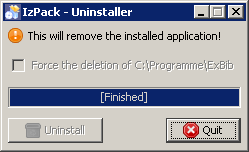
\includegraphics[width=.45\textwidth]{img/uninst2}
  \caption{The Uninstaller Finished}
  \label{fig:uninst2}
\end{figure}

The uninstaller shows a progress bar (see figure~\ref{fig:uninst2}).
When the uninstaller has finished its work all files and directories
installed with the installer have been removed. Modified and other
files are left untouched.

You can uninstall \ExBib\ by simply removing the installation
directory.%
\index{installation directory|(}\index{directory installation|(} But
this is unsave since all local modification are lost as well.

%%*****************************************************************************
%% $Id: cli-exbib.tex,v 0.00 2008/05/02 17:03:28 gene Exp $
%%*****************************************************************************
%% Author: Gerd Neugebauer
%%-----------------------------------------------------------------------------


%------------------------------------------------------------------------------
\section{Running \ExBib}
%@author Gerd Neugebauer

Currently \ExBib\ can be run from the command line. In this respect it
is more or less identical to \BibTeX\ and can be used as a plug-in
replacement. In addition the features of \BibTeX~8 are present as
well. The marks in the margin indicate where the different features
are coming from.

%-----------------------------------------
%
%The following sample show a simple invocation of \ExBib\ without any
%command line arguments.
%
%{\lstset{morecomment=[l]{*}}%
%\begin{lstlisting}{}
%# exbib
%This is exbib, Version 0.0 (TeX compatibility mode)
%**\relax
%
%*\end
%
%No pages of output.
%Transcript written on ./texput.log.
%\end{lstlisting}}
%
%In this case \ExTeX\ enters interaction with the user and asks for an
%input file. This is indicated by the two asterisks. We have entered
%\macro{relax} here to indicate that we are not willing to pass in a
%file name. The \ExTeX\ system asks us to enter some command --
%indicted by the single asterisk. Here we have entered \macro{end} to
%indicate that we want to finish the processing. Thus \ExTeX\ 
%terminates normally.
%
%\INCOMPLETE
%
%{\lstset{morecomment=[l]{*}}%
%\begin{lstlisting}{}
%# extex plain
%This is ExTeX, Version 0.0 (TeX compatibility mode)
%(plain Preloading the plain format: codes, registers, parameters, fonts,
%more fonts, macros, math definitions, output routines, hyphenation(hyphen))
%*\dump
%Beginning to dump on file plain.fmt
%
%*\end
%
%No pages of output.
%Transcript written on ./plain.log.
%\end{lstlisting}}
%
%
%--------------------------------
%The invocation of the executable \Prog{extex} can be controlled by
%large number of command line arguments. Those command line arguments
%are described in the following list:
%
%\begin{description}
%\item[\Arg{code}]\ \\
%  This parameter contains \ExTeX\ code to be executed directly. The
%  execution is performed after any code specified in an input file. On
%  the command line the code has to start with a backslash. This
%  restriction does not hold for the property settings.
%
%  This command line argument sets the property \Property{extex.code}
%  
%\item[\Arg{file}]\ \\
%  This parameter contains the file to read from. A file name may not
%  start with a backslash or an ambercent. It has no default.
%
%  This command line argument sets the property \Property{extex.file}.
%  
%\item[\CLI{-} \Arg{file}]\ \\
%  This parameter terminates the normal processing of arguments. The
%  next argument -- if present -- is interpreted as input file. With
%  this construction it is possible to process an input file which
%  starts with one of the special characters \verb|\| or \verb|&|.
%
%  This command line argument sets the property \Property{extex.file}
%  if a file argument is present.
%
%\item[\CLI{configuration} \Arg{resource}]\ \\
%  This parameter contains the name of the configuration resource to
%  use. This configuration resource is sought on the class path.
%  
%  This command line argument sets the property \Property{extex.config}.
%  
%\item[\CLI{copyright}]\ \\
%  This command line option produces a copyright notice on the standard
%  output stream and terminates the program afterwards.
%
%\item[\tt\&\Arg{format}]\index{\&}
%\item[\CLI{fmt} \Arg{format}]\ \\
%  This parameter contains the name of the format to read. An empty
%  string denotes that no format should be read. This is the default.
%
%  This command line argument sets the property \Property{extex.format}.
%  
%\item[\CLI{debug} \Arg{spec}]\ \\
%  This command line parameter can be used to instruct the program to
%  produce debugging output of several kinds. The debug output is
%  written to the log file. The specification \Arg{spec} is interpreted
%  left to right. Each character is interpreted according to the
%  following table:
%
%  \begin{tabular}{lp{.4\textwidth}l}\toprule
%    \textit{Spec}& \textit{Description}& \textit{See} \\\midrule
%    F& 	This specifier contains the indicator whether or not to trace
%    the searching for input files. & 	\Property{extex.trace.input.files}\\
%    f& 	This specifier contains the indicator whether or not to trace
%    the searching for font files.&      \Property{extex.trace.font.files}\\
%    M& 	This specifier contains the indicator whether or not to trace
%    the execution of macros.&	 	\Property{extex.trace.macros}\\
%    T& 	This specifier contains the indicator whether or not to trace
%    the work of the tokenizer.& 	\Property{extex.trace.tokenizer}\\
%    \bottomrule
%  \end{tabular}
%
%  The following example shows a possible invocation with this
%  parameter: 
%\begin{lstlisting}{}
%# extex -debug FfMT abc.tex
%This is ExTeX, Version 0.0 (TeX compatibility mode)
%...
%\end{lstlisting}
%  
%\item[\CLI{halt-on-error}]\ \\
%  This parameter contains the indicator whether the processing should
%  halt after the first error which has been encountered.
%
%  This command line argument sets the property \Property{extex.halt.on.error}.
%  
%\item[\CLI{help}]\ \\
%  This command line option produces a short usage description on the
%  standard output stream and terminates the program afterwards.
%  
%\item[\CLI{ini}]\ \\
%  If set to true then act as ini\TeX.\index{initex@ini\TeX} In this
%  case no format has to be preloaded. All parameters are set to the
%  "`factory settings"'.
%
%  This command line argument sets the property \Property{extex.ini}.
%
%  The following example shows a possible invocation with this
%  parameter: 
%\begin{lstlisting}{}
%# extex -ini abc.tex
%This is ExTeX, Version 0.0 (TeX compatibility mode)
%...
%\end{lstlisting}
%  
%\item[\CLI{interaction} \Arg{mode}]\ \\
%  This parameter contains the interaction mode. possible values are
%  the numbers 0\dots3 and the symbolic names \Mode{batchmode} (0),
%  \Mode{nonstopmode} (1), \Mode{scrollmode} (2), and
%  \Mode{errorstopmode} (3).
%
%  This command line argument sets the property \Property{extex.interaction}.
%  
%  The following example shows a possible invocation with this
%  parameter:
%\begin{lstlisting}{}
%# extex -interaction batchmode abc.tex
%This is ExTeX, Version 0.0 (TeX compatibility mode)
%...
%\end{lstlisting}
%
%\item[\CLI{job-name} \Arg{name}]\ \\
%  This parameter contains the name of the job. It is overwritten if a
%  file is given to read from. In this case the base name of the input
%  file is used instead.
%
%  This command line argument sets the property \Property{extex.jobname}.
%  
%\item[\CLI{language} \Arg{language}]\ \\
%  This parameter contains the name of the locale to be used for the
%  messages.
%
%  This command line argument sets the property \Property{extex.lang}.
%  
%\item[\CLI{output} \Arg{format}]\ \\
%  This parameter contains the output format. This logical name is
%  resolved via the configuration.
%
%  This command line argument sets the property \Property{extex.output}.
%
%  The following example shows a possible invocation with this
%  parameter: 
%\begin{lstlisting}{}
%# extex -output pdf abc.tex
%This is ExTeX, Version 0.0 (TeX compatibility mode)
%\end{lstlisting}
%  
%\item[\CLI{progname} \Arg{name}]\ \\
%  This parameter can be used to overrule the name of the program shown
%  in the banner and the version information.  The following example
%  shows a possible invocation and the resulting output:
%
%\begin{lstlisting}{}
%# extex -progname XeTxE -version
%This is XeTxE, Version 0.0 (1.4.2_06)
%#
%\end{lstlisting}
%
%  This command line argument sets the property \Property{extex.progname}.
%  
%\item[\CLI{texinputs} \Arg{path}]\ \\
%  This parameter contains the additional directories for searching
%  \ExTeX\ input files.  The directories are separated by the
%  system-dependant separator.  This separator is a colon (\verb|:|) on
%  Unix\index{Unix} and the semicolon (\verb|;|) on
%  Windows\index{Windows}.
%  
%  This command line argument sets the property
%  \Property{extex.texinputs}.
%  
%\item[\CLI{texmfoutputs} \Arg{dir}]\ \\
%  This parameter contains the name of the property for the fallback if
%  the output directory fails to be writable.
%  
%  This command line argument sets the property
%  \Property{extex.outputdir.fallback}.
%  
%\item[\CLI{texoutputs} \Arg{dir}]\ \\
%  This parameter contain the directory where output files should be
%  created.
%
%  This command line argument sets the property \Property{extex.outputdir}.
%  
%\end{description}
%

\subsection{Command Line Parameters}
%@author Gerd Neugebauer

\subsubsection{The Aux File}

\begin{description}
\item[\Arg{file}]\ \\
  This parameter contains the aux file to read from. A file name may not
  start with minus sign. It has no default.
  \begin{lstlisting}{}
    # extex doc.aux
    This is exbib, Version 0.1
  \end{lstlisting}
  
\item[\CLI{} \Arg{file}]
\item[\CLI{-} \Arg{file}]\ \\
  This parameter terminates the intercepts processing of arguments. The
  next argument -- if present -- is interpreted as input file. With
  this construction it is possible to process an input file which
  starts with the special character \verb|-|.
  \begin{lstlisting}{}
    # extex -- doc.aux
    This is exbib, Version 0.1
  \end{lstlisting}

\end{description}

The file name given is used to determine the name of an aux file. This
means that it is either the name of an aux file or the base name which
is augmented by the extension \texttt{.aux} to find the aux file.

The main control information is taken from this aux file. This means
it contains the foloowing items:

\begin{itemize}
\item The database files to consult.
\item The citations to extract.
\item The bst to use for formatting.
\item References to other aux files to consult as well.
\end{itemize}

\subsubsection{Version Information and Help}

\begin{description}
\item[\CLI{-copying}]\ \\
  This command line option produces a copyright notice on the standard
  output stream and terminates the program afterwards.
  \begin{lstlisting}{}
# exbib --copying
                 GNU LESSER GENERAL PUBLIC LICENSE
                      Version 2.1, February 1999
Copyright (C) 1991, 1999 Free Software Foundation, Inc.
    59 Temple Place, Suite 330, Boston, MA  02111-1307  USA
Everyone is permitted to copy and distribute verbatim copies
of this license document, but changing it is not allowed.
[This is the first released version of the Lesser GPL.  It also counts
as the successor of the GNU Library Public License, version 2, hence
the version number 2.1.]
                           Preamble
 The licenses for most software are designed to take away your
freedom to share and change it.  By contrast, the GNU General Public
Licenses are intended to guarantee your freedom to share and change
free software--to make sure the software is free for all its users.
    ...
  \end{lstlisting}

\item[\CLI{h}]
\item[\CLI{?}]
\item[\CLI{-help}]\ \\
  This command line option produces a short usage description on the
  standard output stream and terminates the program afterwards.
  \begin{lstlisting}{}
# exbib --help
This is exbib, Version 0.1
Usage: exbib <options> file
The following options are supported:
        -[-] <file>
                Use this argument as file name -- even when it looks like an option.
        --trad[itional] | -7
                operate in the original 7-bit mode.
        --8[bit] | -8
                force 8-bit mode, no CS file used.
    ...
\end{lstlisting}
  
\item[\CLI{-release}]\ \\
  This command prints the release number to stdout and exits the
  program. This can be used to enable external programs to easily
  determine the version number of \ExBib.
\begin{lstlisting}{}
# exbib --release
0.1
#
\end{lstlisting}

\item[\CLI{-version}]\ \\
  This command line parameter forces that the version information is
  written to standard output and the program is
  terminated.\index{version} The version of \ExBib\ is shown. The
  following example shows a possible invocation and the resulting
  output:
\begin{lstlisting}{}
# exbib --version
This is exbib, Version 0.1
Copyright (C) 2002-2008 Gerd Neugebauer (mailto:gene@gerd-neugebauer.de).
There is NO warranty.  Redistribution of this software is
covered by the terms of the GNU Library General Public License.
For more information about these matters, use the command line
switch -copying.
#
\end{lstlisting}
\end{description}


\subsubsection{Internationalization}

\begin{description}
\item[\CLI{L} \Arg{lang}]
\item[\CLI{-language} \Arg{lang}]\ \\
  This command line option switches the language to the given
  language. The argument is a two-letter ISO code for a language. For
  instance the value \texttt{en} represents English and \texttt{de}
  represents German.

  The language is used to select the appropriate messages for logging
  and error messages. If the given language is not supported English
  is silently used as fallback.
\begin{lstlisting}{}
# exbib --language de --help
Dies ist exbib, Version 0.1
Copyright (C) 2002-2008 Gerd Neugebauer (mailto:gene@gerd-neugebauer.de).
There is NO warranty.  Redistribution of this software is
covered by the terms of the GNU Library General Public License.
For more information about these matters, use the command line
switch -copying.
#
\end{lstlisting}
\end{description}


\subsubsection{Configurations}

\ExBib\ is highly configurable. The whole system is assembled from
components at run time. The assembly is controlled from a set of
configuration files. There is one central configuration file which
acts as entry point.

\begin{description}
\item[\CLI{c} \Arg{config}]
\item[\CLI{-configuration} \Arg{config}]\ \\
  Set the configuration file to be used for assenbling \ExBib. The
  default is the configuration \texttt{exbib}.
\begin{lstlisting}{}
# exbib --configuration bibtex099 doc.aux
This is exbib, Version 0.1
...
\end{lstlisting}

\item[\CLI{-bibtex}]
\item[\CLI{-strict}]\ \\
  Use the configuration \texttt{bibtex099} for assembling \ExBib.
\begin{lstlisting}{}
# exbib --bibtex doc.aux
This is exbib, Version 0.1
...
\end{lstlisting}
\end{description}

The following configurations are present in the distribution.

\begin{description}
\item[exbib]\ \\
  This is the default configuration which includes all features
  described in this reference manual.
\item[bibtex099]\ \\
  This is the configuration for backward compatibility. It emulates
  the features of \BibTeX~0.99c as closely as possible. The extended
  features of \ExBib\ are not present in this configuration.
\end{description}

\subsubsection{Encodings}

The internal representation of characters uses Unicode. In general it
is necessary to translate from and to the internal representation when
reading and writing files. For this purpose the encodings to be used
can be configured.

The default is to use the default encoding for the platform \ExBib\ is
currently running. Thus it is not necessary to specify an encoding at
all.

It is guaranteed that at least the following encodings are present on
your system:

\begin{description}
\item[US-ASCII] 
  Seven-bit ASCII.
\item[ISO-8859-1] 
  ISO Latin Alphabet 1
\item[UTF-8] 
  Eight-bit UCS Transformation Format.
\item[UTF-16BE] 
  Sixteen-bit UCS Transformation Format in big-endian byte order.
\item[UTF-16LE] 
  Sixteen-bit UCS Transformation Format in little-endian byte order.
\item[UTF] Sixteen-bit UCS Transformation Format; the byte order
  identified by an optional byte-order mark.
\end{description}

The following list has been obtained at the time of writing this
document (on a Windows system):

\noindent
\begin{multicols}5\obeylines\scriptsize\parindent=0pt
  Big5
  Big5-HKSCS
  EUC-JP
  EUC-KR
  GB18030
  GB2312
  GBK
  IBM-Thai
  IBM00858
  IBM01140
  IBM01141
  IBM01142
  IBM01143
  IBM01144
  IBM01145
  IBM01146
  IBM01147
  IBM01148
  IBM01149
  IBM037
  IBM1026
  IBM1047
  IBM273
  IBM277
  IBM278
  IBM280
  IBM284
  IBM285
  IBM297
  IBM420
  IBM424
  IBM437
  IBM500
  IBM775
  IBM850
  IBM852
  IBM855
  IBM857
  IBM860
  IBM861
  IBM862
  IBM863
  IBM864
  IBM865
  IBM866
  IBM868
  IBM869
  IBM870
  IBM871
  IBM918
  ISO-2022-CN
  ISO-2022-JP
  ISO-2022-JP-2
  ISO-2022-KR
  ISO-8859-1
  ISO-8859-13
  ISO-8859-15
  ISO-8859-2
  ISO-8859-3
  ISO-8859-4
  ISO-8859-5
  ISO-8859-6
  ISO-8859-7
  ISO-8859-8
  ISO-8859-9
  JIS\_X0201
  JIS\_X0212-1990
  KOI8-R
  KOI8-U
  Shift\_JIS
  TIS-620
  US-ASCII
  UTF-16
  UTF-16BE
  UTF-16LE
  UTF-32
  UTF-32BE
  UTF-32LE
  UTF-8
  windows-1250
  windows-1251
  windows-1252
  windows-1253
  windows-1254
  windows-1255
  windows-1256
  windows-1257
  windows-1258
  windows-31j
  x-Big5-Solaris
  x-euc-jp-linux
  x-EUC-TW
  x-eucJP-Open
  x-IBM1006
  x-IBM1025
  x-IBM1046
  x-IBM1097
  x-IBM1098
  x-IBM1112
  x-IBM1122
  x-IBM1123
  x-IBM1124
  x-IBM1381
  x-IBM1383
  x-IBM33722
  x-IBM737
  x-IBM834
  x-IBM856
  x-IBM874
  x-IBM875
  x-IBM921
  x-IBM922
  x-IBM930
  x-IBM933
  x-IBM935
  x-IBM937
  x-IBM939
  x-IBM942
  x-IBM942C
  x-IBM943
  x-IBM943C
  x-IBM948
  x-IBM949
  x-IBM949C
  x-IBM950
  x-IBM964
  x-IBM970
  x-ISCII91
  x-ISO-2022-CN-CNS
  x-ISO-2022-CN-GB
  x-iso-8859-11
  x-JIS0208
  x-JISAutoDetect
  x-Johab
  x-MacArabic
  x-MacCentralEurope
  x-MacCroatian
  x-MacCyrillic
  x-MacDingbat
  x-MacGreek
  x-MacHebrew
  x-MacIceland
  x-MacRoman
  x-MacRomania
  x-MacSymbol
  x-MacThai
  x-MacTurkish
  x-MacUkraine
  x-MS950-HKSCS
  x-mswin-936
  x-PCK
  x-UTF-16LE-BOM
  X-UTF-32BE-BOM
  X-UTF-32LE-BOM
  x-windows-50220
  x-windows-50221
  x-windows-874
  x-windows-949
  x-windows-950
  x-windows-iso2022jp
\end{multicols}

The following command line options are related to encodings:

\begin{description}
\item[\CLI{-availableCharsets}]\ \\
  This instruction lists the available character sets on standard
  output and exits the program.
\begin{lstlisting}{}
# exbib --availableCharsets
Big5
Big5-HKSCS
EUC-JP
EUC-KR
GB18030
GB2312
GBK
IBM-Thai
IBM00858
IBM01140
...
\end{lstlisting}

\item[\CLI{E} \Arg{enc}]
\item[\CLI{-bib-encoding} \Arg{enc}]
\item[\CLI{-bib.encoding} \Arg{enc}]\ \\
  Set the configuration for reading bib database files. The encoding
  needs to be a valid character set.
\begin{lstlisting}{}
# exbib --bib-encoding=UTF8 doc.aux
...
\end{lstlisting}

\item[\CLI{e} \Arg{enc}]
\item[\CLI{-encoding} \Arg{enc}]\ \\

  \INCOMPLETE
\begin{lstlisting}{}
# exbib --encoding=UTF8 doc.aux
...
\end{lstlisting}

\end{description}
%        --e[ncoding] | -e <enc>
%        	Nutze das gegebene Encoding f�r die Ausgabedatei.

\subsubsection{CS Files}

\begin{description}
\item[\CLI{-csfile} \Arg{csfile}]\ \\

  \INCOMPLETE
\begin{lstlisting}{}
# exbib --csfile=iso8859-7.csf doc.aux
...
\end{lstlisting}
%        --cs[file] <csfile>
%        	Nutze das csf zur Definition von Zeichen und Sortierung.

\item[\CLI{7}]
\item[\CLI{-traditional}]\ \\
  \INCOMPLETE
\begin{lstlisting}{}
# exbib --traditional doc.aux
...
\end{lstlisting}
%        --trad[itional] | -7
%        	arbeite im originalen 7-Bit-Modus.

\item[\CLI{8}]
\item[\CLI{-8bit}]\ \\
  \INCOMPLETE
\begin{lstlisting}{}
# exbib --8bit doc.aux
...
\end{lstlisting}
%        --8[bit] | -8
%        	Erzwinge  8-Bit-Modus, es wird keine CS-Datei eingesetzt.
\end{description}

\subsubsection{Redirecting Output}

\begin{description}
\item[\CLI{l} \Arg{file}]
\item[\CLI{-logfile} \Arg{file}]\ \\
  This option redirects the log output to the given file. The default
  name of the log file is derived from the base name of the aux file
  by appending \texttt{.blg}. This option overwrites this default.
  behaviour.
\begin{lstlisting}{}
# exbib --logfile=my.log doc.aux
...
\end{lstlisting}

  If the given file name is the value \texttt{-} then the output is
  sent to stdout.
\begin{lstlisting}{}
# exbib --logfile=- doc.aux
...
\end{lstlisting}

  If the given file name is empty then the log output is discarted.
\begin{lstlisting}{}
# exbib --logfile= doc.aux
...
\end{lstlisting}

\item[\CLI{o} \Arg{file}]
\item[\CLI{-output} \Arg{file}]
\item[\CLI{-outfile} \Arg{file}]\ \\
  This option redirects the output to the given file. The default
  name of the output file is derived from the base name of the aux file
  by appending \texttt{.bbl}. This option overwrites this default.
  behaviour.
\begin{lstlisting}{}
# exbib --outfile=my.out doc.aux
...
\end{lstlisting}

  If the given file name is the value \texttt{-} then the output is
  sent to stdout.
\begin{lstlisting}{}
# exbib --outfile=- doc.aux
...
\end{lstlisting}

  If the given file name is empty then the output is discarted.
\begin{lstlisting}{}
# exbib --outfile= doc.aux
...
\end{lstlisting}

\end{description}


\subsubsection{Changing the Style}

\begin{description}
\item[\CLI{b} \Arg{style}]
\item[\CLI{-bst} \Arg{style}]\ \\
  This option sets the name of the bib style to be used. The bib style
  is normally read from the aux file. This instruction overrules
  whatever the aux file contains.
\begin{lstlisting}{}
# exbib --bst=alpha doc.aux
...
\end{lstlisting}

\end{description}

\subsubsection{min crossrefs}

\begin{description}
\item[\CLI{M} \Arg{n}]
\item[\CLI{-min-crossrefs} \Arg{n}]
\item[\CLI{-min.crossrefs} \Arg{n}]
\item[\CLI{-min\_crossrefs} \Arg{n}]\ \\
  This option sets the minimum number of crossreferences before an
  entry is not collaped.
\begin{lstlisting}{}
# exbib --min-crossrefs=4 doc.aux
...
\end{lstlisting}

\end{description}

\subsubsection{Naming the Program}

\begin{description}
\item[\CLI{p} \Arg{name}]
\item[\CLI{-progname} \Arg{name}]
\item[\CLI{-program-name} \Arg{name}]
\item[\CLI{-program.name} \Arg{name}]\ \\
  This option sets the name of the porogram. Thus it is possible to
  influence how the program calls itself in logging and error messages
  from outside .
\begin{lstlisting}{}
# exbib --progname=BibTeX doc.aux
This is BibTeX, Version 0.1
...
\end{lstlisting}

\end{description}


\subsubsection{Tracing and Debugging}

\begin{description}
\item[\CLI{d} \Arg{mode}]
\item[\CLI{-debug} \Arg{mode}]\ \\
\end{description}
%        --d[ebug] | -d
%        	Arbeite im Debug-Modus.

\begin{description}
\item[\CLI{q}]
\item[\CLI{-terse}]
\item[\CLI{-quiet}]\ \\
  This option switches the operation to quiet mode. Nearly all
  informative messages are suppressed oin stdanard output.
  Nevertheless they can be found in the log file -- if one is written.
\begin{lstlisting}{}
# exbib --quiet doc.aux
#
\end{lstlisting}

\item[\CLI{t}]
\item[\CLI{-trace}]\ \\
  Write a detailed log of internal operations to the log file.  The
  tracing can be very useful when you try to understand the operations
  of the bst interpreter.
  
  Note that this option can drastically decrease the performance of
  operation.
\begin{lstlisting}{}
# exbib --trace doc.aux
This is BibTeX, Version 0.1
...
\end{lstlisting}

\item[\CLI{v}]
\item[\CLI{-verbose}]\ \\
  This option switches the operation to verbose mode. Some more
  informative messaged might be presented during the operation.
\begin{lstlisting}{}
# exbib --verbose doc.aux
#
\end{lstlisting}
\end{description}


\subsubsection{Ignored Options}

\IM{8x} Several command line options have a special meaning in
\BibTeX~8 without a corresponding pendant in \ExBib. Most of them are
related to memory allocation. In \ExBib\ the memory allocation is
fully dynamic and no predefined sizes are necessary.

For compatibility those options are silently ignored:
\begin{description}
\item[\CLI{s}]
\item[\CLI{-statistics}]
\item[\CLI{B}]
\item[\CLI{-big}]
\item[\CLI{H}]
\item[\CLI{-huge}]
\item[\CLI{W}]
\item[\CLI{-wolfgang}]
\item[\CLI{-mcites}]
\item[\CLI{-mentints}]
\item[\CLI{-mentstrs}]
\item[\CLI{-mfields}]
\item[\CLI{-mpool}]
\item[\CLI{-mstrings}]
\item[\CLI{-mwizfuns}]
\end{description}


\subsection{Abbreviation of Long Parameters}
%@author Gerd Neugebauer

Command line parameters can be abbreviated up to a unique prefix --
and sometimes even more. Thus the following invocations are
equivalent:

\begin{verbatim}
  exbib --vers
  exbib --versi
  exbib --versio
  exbib --version  
\end{verbatim}


\endinput
%
% Local Variables: 
% mode: latex
% TeX-master: nil
% End: 
%        --r[elease]
%        	Zeige die Versionsnummer und beende das Programm.


\endinput
%
% Local Variables: 
% mode: latex
% TeX-master: "../exbib-users"
% End: 
